Lo String Matching Algorithm Research Tool, da qui in poi SMART \cite{smart}, è un tool dedicato ai ricercatori e a gli studenti di algoritmi di confronto fra stringhe. Il tool offre un ambiente versatile, scalabile e facilmente integrabile con nuovi algoritmi per effettuare considerazioni qualitative nella cornice dei problemi derivati dalla più ampia materia del \textit{pattern matching}. In generale, SMART propone un framework di lavoro adatto a testare, progettare, valutare e comprendere le soluzioni del problema del confronto fra stringhe. 

\vspace{3mm}

Il tool è stato sviluppato da un gruppo accademico internazionale \cite{smartHomepage}, il quale ha successivamente rilasciato il codice sorgente dell'applicativo su GitHub in una repository pubblica. Il tool ha successivamente ricevuto una moderata documentazione ai fini di coadiuvare i futuri sviluppatori che intendessero estendere le funzionalità del tool o, più banalmente, integrare nuovi algoritmi di confronto fra stringhe \cite{smartHelp}.

\vspace{3mm}

E' possibile utilizzare SMART in ambiente Windows, MAC OS X e Linux. Per semplicità, si è deciso di utilizzare una macchina virtualizzata montata con Ubuntu 64bit. L'ambiente di lavoro barebones e Unix-based ha permesso al tool di lavorare al massimo dell'efficienza e senza alcun disguido di natura tecnica, che avrebbero potuto aver luogo in contesti non-Unix, come Windows e MAC OS X, soprattutto in termini di compatibilità con librerie e dipendenze di cui SMART fa ampiamente uso.

\section{Funzionamento di SMART}

\begin{figure}[ht!]
    \centering
    \tmpframe{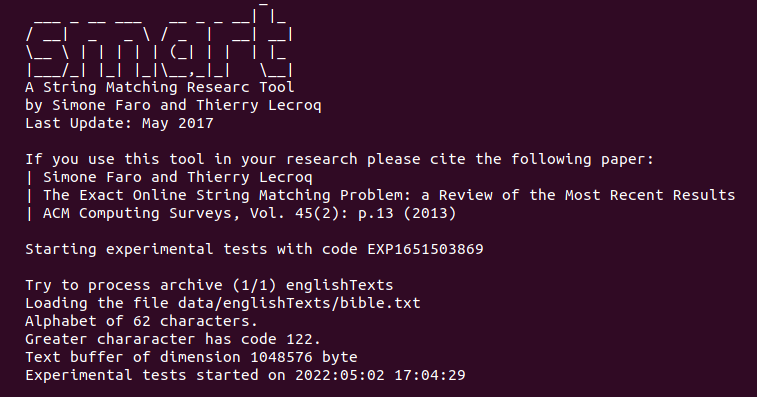
\includegraphics[width=6in]{Figure/smartWelcome.png}}
    \caption{Schermata di benvenuto del tool SMART.}
    \label{fig:esempio}
\end{figure}

Ad alto livello, il tool SMART:

\begin{itemize}
    \item Permette di selezionare al più $N$ algoritmi $A+$, dove:
    \begin{itemize}
        \item $A+$ è un algoritmo che sia testato, funzionante e \textit{valido}. Un algoritmo $A$ non testato, funzionante o valido non può essere selezionato. Una volta testato tramite gli appropriati strumenti offerti dal tool, un simbolo $+$ viene utilizzato per indicare la traslazione di stato da algoritmo non selezionabile $A$ ad algoritmo selezionabile $A+$.
        \item $N$ è il numero di algoritmi disponibili. In particolare, $N$ non coincide necessariamente con i sorgenti degli algoritmi presenti nel filesystem del tool, bensì con il numero di algoritmi presenti nella cartella \verb|~root/sources/algos| al momento della compilazione e del bundling tramite \verb|Makefile|. Il processo è descritto nel dettaglio in seguito.
    \end{itemize}
    \item Permette di selezionare uno o più testi $T$ su cui lanciare la computazione. I testi, incapsulati in file TXT, sono fra i più variegati:
    \begin{itemize}
        \item Testi accademici o letterari scritti in linguaggio naturale e in lingue diverse. Di default, SMART offre testi in lingua italiana, inglese, francese e cinese. Si tratta di testi narrativi più o meno lunghi, oppure di articoli accademici di dominio pubblico. La lunghezza di questi testi si aggira sulle centinaia di migliaia di parole.
        \item Descrizioni del genoma. Insiemi di stringhe su alfabeti DNA o PROT. 
    \end{itemize}
    \item Permette di selezionare l'upper bound e il lower bound dei pattern da riscontrare nelle sequenze. In generale, SMART confronta le stringhe in input in funzione dei loro pattern costituenti: è possibile, dunque, specificare una lunghezza minima e massima dei suddetti pattern; all'esecuzione, il tool incrementerà la lunghezza dei pattern in maniera esponenziale (ad esempio, potrebbe iniziare confrontando le stringhe con pattern di lunghezza 2, poi 4, 8, 16, 32 e così via). E' anche possibile determinare specifiche regioni di testo sulla quale ricercare i pattern.
    \item Una volta selezionato almeno $1$ algoritmo $A+$ e almeno un testo $T$, ed eventualmente aver definito parametri limitativi sui pattern da rilevare nelle stringhe accolte, è possibile lanciare l'applicativo. Il terminale verrà popolato da barre di caricamento sufficientemente descrittive che segnaleranno l'avanzamento della computazione. Una volta conclusa, SMART indicizzerà l'esperimento con l'attuale $timestamp$ seguendo una nomenclatura precisa (es. $EXP20220203$). 
    
    \begin{figure}[ht!]
    \centering
    \tmpframe{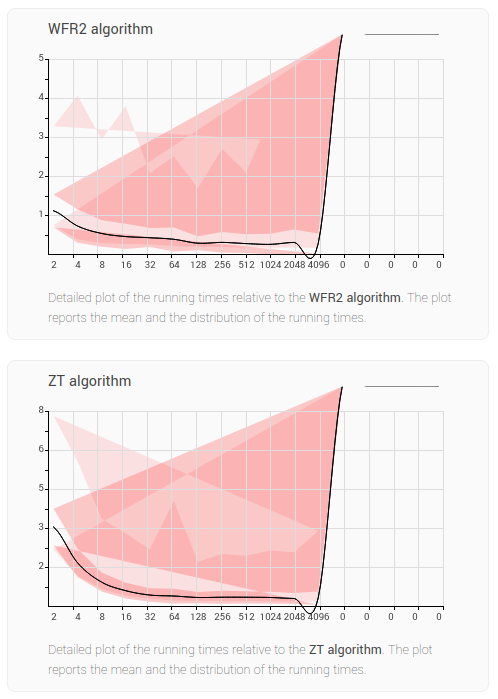
\includegraphics[width=5in]{Figure/smartDistribution.png}}
    \caption{Dettaglio di un grafico sulla \textit{Distribution} generato da SMART relativo a due algoritmi: WFR2 e ZT.}
    \label{fig:esempio}
\end{figure}
    
    Il tool creerà una cartella in \verb|/results| col nome dell'esperimento e inserirà in quest'ultima i risultati ottenuti sotto forma di alcune pagine HTML elaborate con CSS e JavaScript. La pagina conterrà, essenzialmente, dei grafici informativi sulla computazione appena effettuata, dando spazio a considerazioni di natura qualitativa e comparativa degli algoritmi $A+$ selezionati in funzione dei testi $T$ impiegati.
\end{itemize}

\begin{figure}[ht!]
    \centering
    \tmpframe{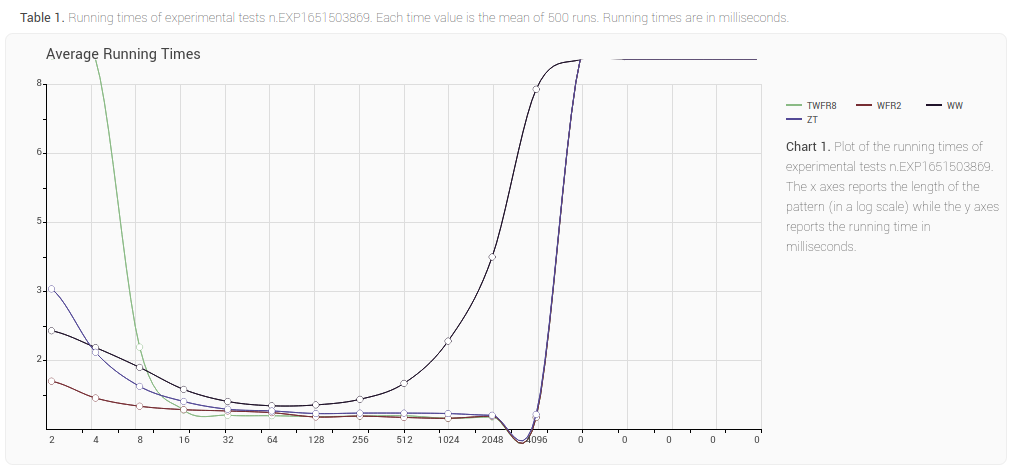
\includegraphics[width=6in]{Figure/smartGraph.png}}
    \caption{Dettaglio di un grafico sull'\textit{Average Running Time} generato da SMART.}
    \label{fig:esempio}
\end{figure}

\subsection{Installazione e compilazione}

Analizzando il codice sorgente di SMART su GitHub \cite{smartGithub} è possibile delineare il funzionamento sia ad alto livello che a basso livello del tool. In generale, gli sviluppatori hanno previsto un processo di installazione immediato: è sufficiente infatti clonare la repository tramite GitHub ed avviare il processo di compilazione e bundling tramite \verb|Makefile|: 

\begin{verbatim}
https://github.com/smart-tool/smart.git
cd smart-tool
./makefile
\end{verbatim}

E' importante osservare che è necessario ricompilare tramite \verb|Makefile| ogni qual volta s'intende integrare un nuovo algoritmo. Infatti, il processo di bundling è esteso alle sotto-directory della \verb|~root|, inclusa la folder \verb|/bin|, che conterrà i file binari di output degli algoritmi. In generale, il filesystem di SMART è così strutturato:

\subsection{Struttura del filesystem}

\begin{itemize}
    \item \verb|~root|: Contiene una serie di eseguibili extension-less lanciabili tramite terminale, fra cui \verb|./SMART| e \verb|./SELECT|. Un ulteriore eseguibile è disponibile per verificare la correttezza dei nuovi algoritmi da integrare nel tool.
    \begin{itemize}
        \item \verb|./SMART|: E' il core dell'applicativo. Da linea di comando, ammette un insieme di opzioni che permettono di descrivere l'input del programma, l'alfabeto utilizzato, la lunghezza massima dei pattern da ricercare nelle stringhe, nonché ulteriori flag opzionali per confronti più specializzati.
        \item \verb|./SELECT|: analogamente all'eseguibile SMART, ammette una serie di opzioni che hanno l'obiettivo di determinare gli algoritmi da utilizzare quando si lancerà il prossimo confronto con SMART. I comandi ammessi, fra gli altri, sono \verb|-show| (stampa un elenco esaustivo degli algoritmi selezionabili), \verb|-none| (deseleziona tutti gli algoritmi), \verb|-all| (seleziona tutti gli algoritmi) e \verb|[ALGO_NAME]| (seleziona uno specifico algoritmo, a patto che sia presente nella cartella \verb|/algos|. Il comando \verb|-which| permette di identificare gli algoritmi attualmente selezionati e in procinto di essere computati con la prossima invocazione del comando \verb|./SMART|. Infine, il comando \verb|-add| permette di integrare nuovi algoritmi nel tool: è un comando centrale nel funzionamento ad alto livello di SMART, poiché permette a sviluppatori esterni di estenderne le prospettive computative.
        
        \begin{figure}[ht!]
        \centering
        \tmpframe{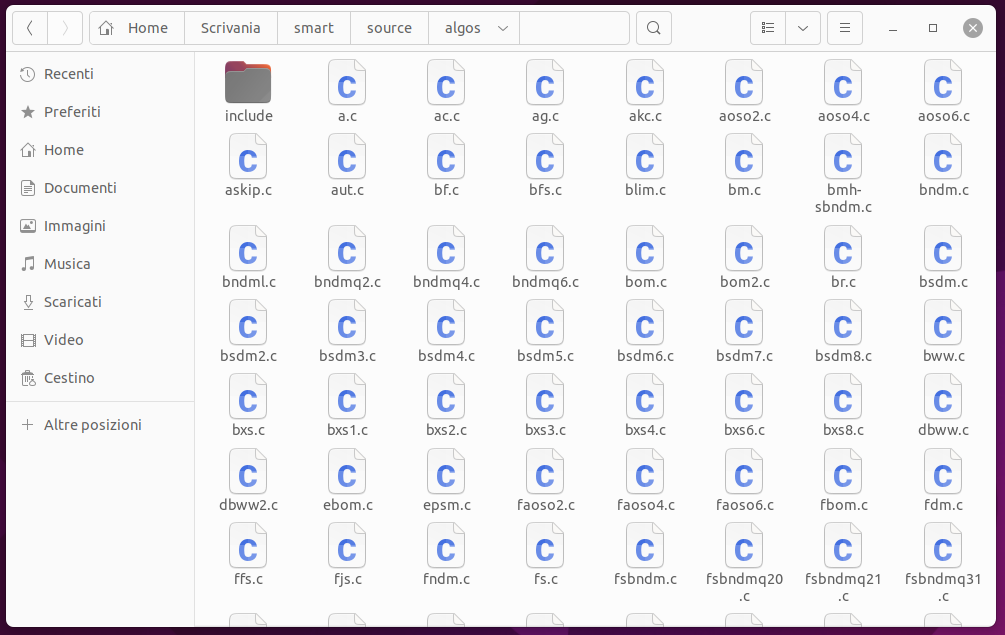
\includegraphics[width=5.5in]{Figure/smartAlgos.png}}
        \caption{Contenuto della cartella ALGOS. L'anteprima non mostra la presenza di una sottocartella BIN, motivo per cui è immediato assumere che l'attuale istanza di SMART non sia stata ancora compilata tramite MAKEFILE.}
        \label{fig:esempio}
        \end{figure}
    \end{itemize}
    La root del filesystem contiene anche file di copyright e guide all'installazione del software.
    \item \verb|/data|: contiene una serie di sottocartelle descrittive dei possibili testi da fornire in input al programma. Ad esempio, la cartella \verb|/data/englishTexts| contiene \verb|bible.text| e \verb|index.txt|. Il primo conterrà il testo grezzo in UTF-8; il secondo conterrà alcune informazioni di indicizzazione del testo per permettere all'applicativo di utilizzarlo come input. Di default, infatti, il testo in inglese di riferimento è la trascrizione della Bibbia; invece, i testi in italiano di riferimento sono, fra gli altri, l'Orlando furioso, la Divina Commedia e le Ultime lettere di Jacopo Ortis. Il file \verb|data/italianTexts/index.txt| sarà così strutturato:
    
    \begin{sexylisting}{data/italianTexts/index.txt}
La divina commedia
Dante Aligheri (1307)
[url della fonte]
#la_divin.txt#
551,9 kB

Orlando furioso
Ludovico Ariosto (1532)
[url della fonte]
#orlando_.txt#
1,5 MB

Ultime lettere di Jacopo Ortis
Ugo Foscolo (1817)
[url della fonte]
#ultime_l.txt#
281,2 kB

    \end{sexylisting}
    \item \verb|/results|: contiene tante sottocartelle quanti gli esperimenti (eg. \textit{computazioni}) elaborati tramite SMART. I nomi delle cartelle seguono una nomenclatura univoca, come descritto in precedenza, e associano ad ogni esperimento un preciso identificativo, determinato dal timestamp.
    \item \verb|/source|: contiene i file sorgenti C del core del software (ad esempio \verb|./smart.c| per l'eseguibile \verb|./SMART/|) e degli algoritmi di confronto fra stringhe disponibile. Circa 80 algoritmi sono disponibili di default, e nuovi sono integrabili. In particolare:
    \begin{itemize}
        \item La cartella \verb|/algos| contiene i file sorgenti C degli algoritmi, strutturati in modo specifico al fine di poter essere compatibili col tool. Il \verb|Makefile| di SMART compilerà questi file sorgente C in binari di output. 
        \item La cartella \verb|/bin| contiene i file binari risultato della compilazione dei sorgenti in C di \verb|/algos|. In effetti, questi file binari sono esattamente quelli utilizzati durante i processi computazionali del tool. 
    \end{itemize}
\end{itemize}

\section{Integrazione di nuovi algoritmi}

Per aggiungere un nuovo algoritmo al tool SMART, è necessario creare un file sorgente in C nella cartella \verb|~root/source/algos| e notificare il tool della sua presenza tramite \verb|./select -add [ALGO_NAME]| dopo averlo opportunamente testato e validato tramite le strumentazioni automatiche del tool. 

\vspace{3mm}

Il contenuto del file C dev'essere compatibile con il modo di computare i confronti fra stringhe e le ricerche di pattern di SMART. L'algoritmo può utilizzare $include$ esterni, come librerie e altre forme di dipendenze programmatiche. Il file sorgente può includere una serie di funzioni ausiliare per favorire il riuso e la leggibilità, oppure per motivi di iterazione o ricorsione. Tuttavia, SMART prevede che almeno una funzione (definita come tale) sia presente nel sorgente C, e che questa funzione abbia una firma ben definita.

\begin{figure}[ht!]
    \centering
    \tmpframe{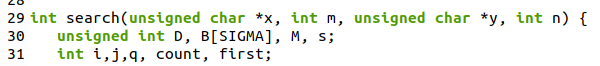
\includegraphics[width=5.5in]{Figure/smartAlgoSign.png}}
    \caption{Firma di un algoritmo predefinito di SMART. Il contenuto della funzione è irrilevante, ma la firma è cruciale.}
    \label{fig:esempio}
\end{figure}

In particolare, la funzione in questione, denominata $search$, deve restituire un intero e accogliere esattamente tre parametri nel seguente ordine:
\begin{itemize}
    \item \verb|unsigned char *x|, pattern da ricercare all'interno del testo $*y$
    \item \verb|int *m|, lunghezza del pattern \verb|*x|
    \item \verb|unsigned char *y|, testo sul quale ricercare il pattern \verb|*x|
    \item \verb|int *n|, lunghezza del testo \verb|*n|
\end{itemize}

Se l'algoritmo non trova alcuna occorrenza del pattern, l'algoritmo dovrà restituire $-1$. In alternativa, dovrà \textbf{restituire \textit{esattamente} il numero di occorrenze del pattern} $*x$ nel testo $*y$.

Il contenuto della funzione è irrilevante, a patto che rispetti i requisiti soprastanti. Questo significa che è possibile usare qualsiasi struttura dati, tecnica algoritmica e metodo di computazione per arrivare all'intero richiesto. La complessità dell'algoritmo è altresì irrilevante e non vincolante all'implementazione o all'integrazione con SMART; sarà difatti compito del tool effettuare le dovete comparazioni degli algoritmi.

\begin{figure}[ht!]
    \centering
    \tmpframe{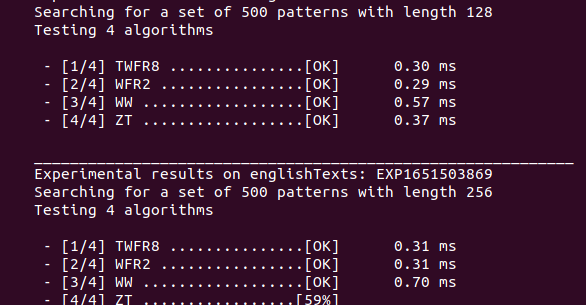
\includegraphics[width=5.5in]{Figure/smartComputing.png}}
    \caption{Porzione di una fase del processo di computazione di SMART. In questa anteprima, SMART sta computando quattro algoritmi: TWFR8, WFR2, WW e ZT. In particolare, sta ricercando un preciso numero di pattern (500) di lunghezza esponenziale (128, 256). Ogni riga presenta il tempo richiesto in millisecondi.}
    \label{fig:esempio}
\end{figure}

E' possibile validare l'algoritmo attraverso il comando \verb|./TEST [ALGO_NAME]|. Il tool tenterà di e, se il numero di occorrenze restituito dall'algoritmo testato coinciderà con l'intero che il tool si aspetta, allora l'algoritmo sarà considerato valido, testato e pienamente funzionante; sarà possibile, a questo punto, integrarlo e selezionarlo tramite \verb|./SELECT|.


\section{Accenni al versioning parallelo di SMART-GUI}

Gli autori del tool SMART, per venire incontro a prerogative di usabilità, hanno deciso di sviluppare una versione parallela che, invece di poter essere utilizzata esclusivamente da linea di comando, sia invece adoperabile tramite un'interfaccia grafica. Questa versione è stata denominata SMART-GUI ed è disponibile su GitHub \cite{smartGUI}. 

\vspace{3mm}

Il funzionamento è del tutto analogo alla sua controparte da terminale. L'unica sostanziale differenza è, appunto, l'introduzione di un'interfaccia grafica, che sostituisce i comandi principali dell'applicativo da CLI, come \verb|./SMART| e \verb|./SMART|, adesso integrati in un'unica finestra sotto forma di riquadri di input, tabs e bottoni interattivi.

\vspace{3mm}

\begin{figure}[ht!]
    \centering
    \tmpframe{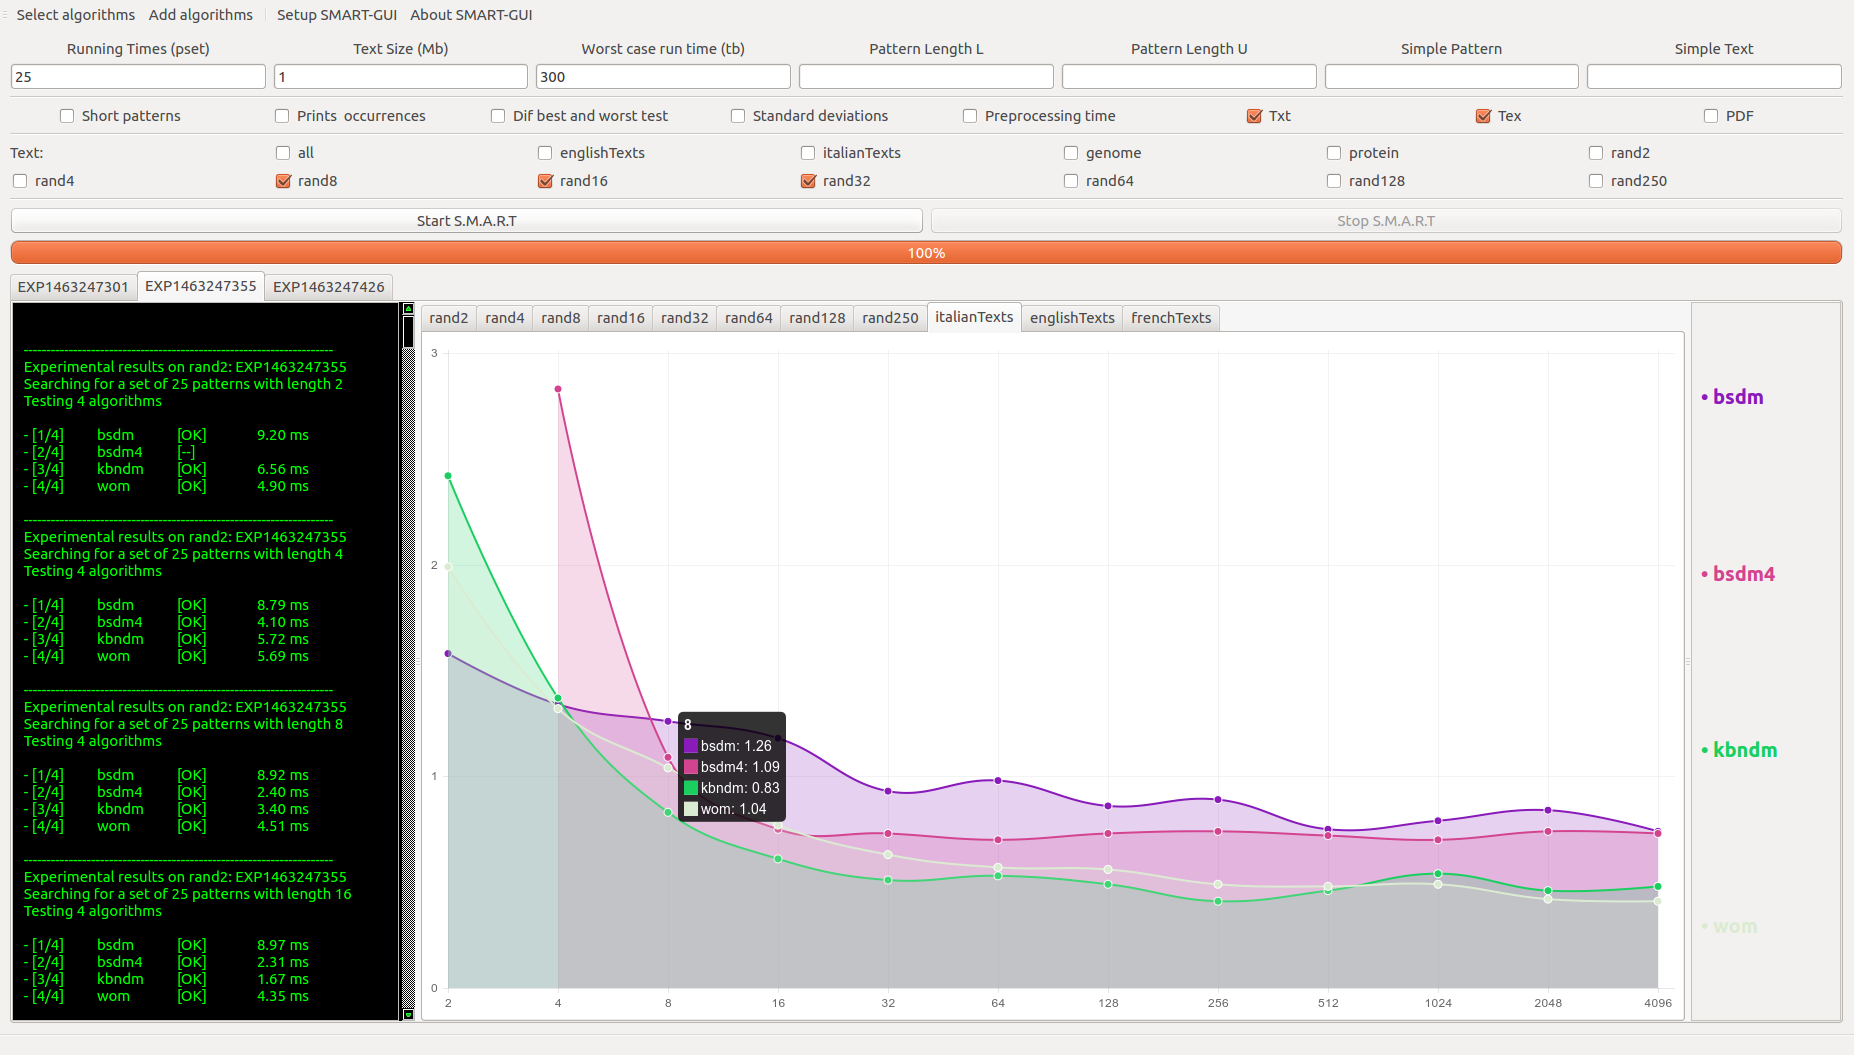
\includegraphics[width=5.5in]{Figure/smartGUI.png}}
    \caption{Anteprima di SMART-GUI.}
    \label{fig:esempio}
\end{figure}

La schermata centrale propone i grafici prodotti dal tool a serguito di un processo computativo. Il lato sinistro, invece, simula le fasi computative proprio come la controparte da terminale del tool. Ulteriori campi di input permettono di specificare i parametri più variegati.

\vspace{3mm}

Tuttavia, l'autore di questa tesi ha individuato empiricamente alcuni problemi di compatibilità relativi alle librerie impiegate per renderizzare l'interfaccia grafica, fra cui \verb|QtLibrary| e \verb|libqtwebkit4|. Potrebbe essere estremamente difficoltoso, o comunque lento e poco efficiente, installare questa versione SMART dotata di interfaccia grafica, per l'utente medio. Numerosi problemi relativi a versioni non più supportate o obsolete delle dipendenze in uso rendono, dunque, la versione da terminale di SMART quella più mantenibile, robusta e funzionante, che risulta altresì immediata e semplice da installare ed utilizzare.

\section{Conclusioni e criticità del software}

Inizialmente, il tool SMART è stato analizzato e studiato come possibile candidato ad ospitare algoritmi come \verb|scMAW|. In generale, si parla di algoritmi che sfruttano le minimal absent words e la metrica LW per indicare la similitudine fra le stringhe oggetto di confronto. Dopo un'attenta analisi e a seguito delle dovute considerazioni, risulta che SMART non sia adeguato né per \verb|scMAW|, né per tutti gli algoritmi che, analogamente a quest'ultimo, 

E' banale osservare come \verb|scMAW| e SMART, in relazione a quanto analizzato in questo Capitolo e nei Capitolo 2 e 3, non possa essere integrabile nel tool secondo i metodi previsti dagli autori. Difatto, come delineato nel Capitolo 4.2, gli algoritmi in via di integrazione devono seguire schemi ben precisi e non posso, almeno nella forma dei parametri accolti e dei tipi restituiti, divergere dalle condizioni vincolanti della piattaforma. Nello specifico, SMART impone la restituzione del numero di occorrenze di un certo pattern in un determinato corpo di testo. Invece, \verb|scMAW| prevede la generazione di un risultato di più ampio respiro, quale un file FASTA.OUT (descritto nel Capitolo 5), contenente indici LW per insiemi ben definiti di stringhe.

Risulta fondamentale osservare come SMART agisca in funzione del numero di occorrenze dei pattern risoluti, mentre gli algoritmi in esame - proprio perché sfruttano l'informazione negativa (nella forma di \textit{absent words} e  simili) piuttosto che quella positiva - sono esclusivamente in grado di fornire un grado di similitudine fra gli elementi input, restringendoli fra l'altro ad un alfabeto specifico, quale quello del genoma. 

Risulta evidente che SMART non sia stato pensato per accogliere algoritmi di questa tipologia. L'implementazione di \verb|scMAW| non può essere adeguata alla forma richiesta dal tool, né sarebbe opportuno tentare di convertire output così distanti e sconnessi fra loro per tentare di assecondare i vincoli del software. 

\vspace{3mm}

Per questi motivi, oltre che per motivi di natura didattica, è stato deciso di realizzare un software ad hoc per integrare algoritmi come quello in esame. 

\vspace{3mm}

In particolare, il tool in sviluppo dovrà essere in grado di elaborare algoritmi che restituiscono un file FASTA.OUT, prendendone in input uno di tipo FASTA e ammettendo esclusivamente l'alfabeto del genoma. Il tool dovrà, similmente a SMART, elaborare dei grafici illustrativi per permettere non solo considerazioni di tipo comparativo sulla qualità degli algoritmi selezionati, ma anche sulla loro correttezza e robustezza in termini degli indici LW restituiti a seguito dell'elaborazione.